\documentclass[smartcities,article,submit,oneauthor]{Definitions/mdpi}

%------------------------------ MDPI internal (no modificar) -----------------------
\firstpage{1}
\makeatletter
\setcounter{page}{\@firstpage}
\makeatother
\pubvolume{1}
\issuenum{1}
\articlenumber{0}
\pubyear{2026}
\copyrightyear{2026}
\datereceived{ }
\dateaccepted{ }
\datepublished{ }

%============================== Paquetes adicionales ===============================
% La clase MDPI ya carga: graphicx, amsmath, amssymb, booktabs, xcolor, colortbl,
% tikz, array, tabularx, hyperref, cleveref, etc. Añadimos solo lo imprescindible.
\usepackage{listings}          % bloques de código "bonitos y elegantes"
\usetikzlibrary{arrows.meta,positioning,shapes.geometric,calc,fit,backgrounds}

% ---- Estilo de listings robusto a acentos y reutilizable ----
\definecolor{codebg}{RGB}{248,249,251}
\definecolor{codeframe}{RGB}{223,227,232}
\definecolor{codekw}{RGB}{170,55,90}
\definecolor{codecom}{RGB}{110,120,130}
\definecolor{codestr}{RGB}{35,120,70}
\definecolor{codenum}{RGB}{150,150,160}

\lstdefinestyle{scn}{
  backgroundcolor=\color{codebg},
  basicstyle=\ttfamily\footnotesize,
  keywordstyle=\color{codekw}\bfseries,
  commentstyle=\color{codecom}\itshape,
  stringstyle=\color{codestr},
  numberstyle=\tiny\color{codenum},
  numbers=left, numbersep=7pt,
  frame=tb, framerule=0.8pt, rulecolor=\color{codeframe},
  breaklines=true, breakatwhitespace=true,
  showstringspaces=false, tabsize=2,
  columns=fullflexible, keepspaces=true,
  aboveskip=8pt, belowskip=6pt,
  literate=%
    {á}{{\'a}}1 {é}{{\'e}}1 {í}{{\'i}}1 {ó}{{\'o}}1 {ú}{{\'u}}1
    {Á}{{\'A}}1 {É}{{\'E}}1 {Í}{{\'I}}1 {Ó}{{\'O}}1 {Ú}{{\'U}}1
    {ñ}{{\~n}}1 {Ñ}{{\~N}}1 {°}{{\textdegree}}1 {→}{{$\rightarrow$}}1
    {≤}{{$\leq$}}1 {≥}{{$\geq$}}1 {β}{{$\beta$}}1 {∨}{{$\vee$}}1
}
\lstset{style=scn}
\lstdefinelanguage{opldat}{ % lenguaje ligero para el .dat de CPLEX/OPL
  morekeywords={hmax,rInf,MaxR,R,S,V,Vs,Cost,Cap,P,L,CVR},
  morecomment=[l]{//}, morecomment=[s]{/*}{*/}, morecomment=[l]{\#},
  sensitive=true, morestring=[b]"
}

% ---- Comandos matemáticos abreviados ----
\newcommand{\Atil}{\tilde{A}}
\newcommand{\Rh}{R_{h}}
\newcommand{\Sh}{S_{h}}
\newcommand{\bin}[1]{\beta\!\left(#1\right)}

%============================== Portada / metadatos ================================
\Title{Plataforma Web para la Generación Automática de Matrices de Conectividad
V2V/V2I en Redes Vehiculares a partir de Escenarios SUMO}

\newcommand{\orcidauthorA}{0000-0000-0000-000X}

\Author{Edison Xavier Espinel Sevilla $^{1,}$*\orcidA{}}

\AuthorNames{Edison Xavier Espinel Sevilla}

\address{%
$^{1}$ \quad Escuela Politécnica Nacional, Quito, Ecuador; edison.espinel@epn.edu.ec}

\corres{Correspondencia: edison.espinel@epn.edu.ec}

% Abstract (sin líneas en blanco)
% Abstract (sin líneas en blanco)
\abstract{(1)~Contexto: el despliegue de unidades de borde de vía (Road Side Units, RSU) constituye uno de los principales desafíos en el diseño de redes vehiculares, debido a que su ubicación determina el nivel de cobertura y conectividad alcanzado por la infraestructura. Los modelos orientados a resolver este problema, tanto exactos como heurísticos, dependen de matrices de conectividad que describan las relaciones entre vehículos y RSU en diferentes instantes y considerando múltiples saltos. La generación de estas matrices representa una etapa compleja, ya que requiere integrar información de movilidad, geometría del entorno y comunicación inalámbrica. (2)~Métodos: en este trabajo se propone una plataforma web para automatizar el proceso de generación de dichos datos, siguiendo el flujo Escenario SUMO~$\rightarrow$~grafo temporal~$\rightarrow$~matrices de conectividad~$\rightarrow$~datos para optimización. El \emph{backend} integra las herramientas de SUMO
(\texttt{netconvert}, \texttt{polyconvert}, \texttt{randomTrips}) junto con un
mecanismo de detección de línea de vista (LoS), considerando los edificios del
entorno como posibles obstáculos. Con esta información se construyen las matrices
de conectividad V2V ($A$) y V2I ($B$), sobre las cuales se aplican operaciones de
álgebra matricial para determinar la conectividad multisalto ($R_h$, $S_h$ y
$D_H$). Por otro lado, el \emph{frontend}, implementado en Streamlit, permite al
usuario definir zonas de estudio sobre mapas reales y consultar los resultados
obtenidos.(3)~Resultados: la plataforma genera los conjuntos de datos requeridos por los modelos de optimización y permite exportarlos tanto en formato OPL/\texttt{.dat}
como mediante estructuras de memoria compatibles con diferentes herramientas de
resolución. El funcionamiento del sistema se evalúa utilizando un escenario real
del Centro Histórico de Quito. (4)~Conclusiones: la herramienta desarrollada establece una conexión entre la simulación vehicular y los modelos de optimización, actuando como una etapa de preprocesamiento que facilita la reutilización de los datos generados en diferentes formulaciones sin necesidad de ejecutar nuevamente la simulación.}

\keyword{VANET; conectividad V2V/V2I; SUMO; Streamlit; matrices de adyacencia;
conectividad multisalto; despliegue de RSU; investigación operativa}

%==================================================================================
\begin{document}

%----------------------------------------------------------------------------------
\section{Introducción}

Las redes vehiculares ad hoc (\emph{Vehicular Ad hoc Network}, VANET) permiten la
comunicación directa entre vehículos (V2V, \emph{Vehicle-to-Vehicle}) y el intercambio
de información con infraestructura fija ubicada en la vía (V2I,
\emph{Vehicle-to-Infrastructure}). Esta infraestructura está formada principalmente
por unidades RSU (\emph{Road Side Units}), generalmente ubicadas en puntos
estratégicos como intersecciones viales. La selección adecuada de sus posiciones
tiene un impacto directo en la cobertura obtenida y en la eficiencia de las rutas de
comunicación dentro de la red. Debido a esto, el problema de ubicación de RSU suele
abordarse mediante técnicas de optimización relacionadas con los modelos clásicos de
localización de instalaciones (\emph{facility location}).

\paragraph{Motivación desde la optimización.} Los enfoques empleados para resolver
el despliegue de infraestructura ---entre ellos \emph{p-median}, \emph{maximal
covering}, \emph{set covering} y modelos estocásticos como el propuesto por
Urquiza-Aguiar~et~al.~\citep{ref-urquiza}--- requieren información previa sobre la
conectividad disponible en la red. En particular, necesitan matrices que representen
qué vehículos pueden comunicarse con cada RSU, en qué instante ocurre dicha conexión
y cuál es la cantidad de saltos involucrados. La obtención de estas matrices implica
integrar diferentes procesos, como la simulación del tráfico vehicular, el análisis
geométrico del entorno y la representación algebraica de las relaciones de
conectividad. A pesar de su importancia, en muchos trabajos de optimización esta
etapa se considera como un dato de entrada previamente disponible, dejando en segundo
plano el procedimiento utilizado para generarla.

\paragraph{Motivación desde el desarrollo de software.} Del lado del software pasa
algo parecido. Hay buenos simuladores (SUMO, Veins, OMNeT++) y buenas librerías de
visualización, pero rara vez aparecen unidos en una sola herramienta web que
acompañe al usuario desde seleccionar un área en el mapa hasta obtener los datos
listos para el \emph{solver}. Ese puente suele resolverse con \emph{scripts}
sueltos, difíciles de reutilizar y de reproducir.

\paragraph{Vacío existente.} Entre ambos mundos queda un hueco concreto: falta una
capa de preprocesamiento que separe con claridad la simulación de tráfico del modelo
de optimización y que entregue las matrices de conectividad de forma automática y
trazable. Ese es el hueco que aborda este trabajo.

\paragraph{Contribuciones.} Las contribuciones de este artículo son:
\begin{enumerate}
\item Una \textbf{plataforma web} que integra SUMO (\emph{backend}) y Streamlit
(\emph{frontend}) en un único flujo reproducible.
\item La \textbf{generación automática} de las matrices de conectividad V2V
(matriz $A$) y V2I (matriz $B$) con detección de línea de vista (LoS) considerando
edificios como obstrucciones.
\item El \textbf{cálculo automático de la conectividad multisalto} ($R_h$, $S_h$,
$D_H$) mediante potencias binarias de la matriz de adyacencia, con su justificación
formal.
\item Un \textbf{algoritmo de selección} de posiciones candidatas para RSU basado
en grado topológico y \emph{clustering} espacial.
\item La \textbf{exportación} de conjuntos de datos listos para modelos de
optimización, ilustrada sobre un caso de estudio real.
\end{enumerate}

Todo el artículo gira en torno a una pregunta: \emph{¿cómo obtener de forma
automática, reproducible y rigurosa los datos que alimentan a un modelo de
optimización de infraestructura vehicular?} La pregunta gemela ---\emph{¿cómo
optimizar el despliegue una vez que se tienen esos datos?}--- se deja para un
trabajo posterior, de modo que cada una pueda tratarse por separado.

%----------------------------------------------------------------------------------
\section{Estado del Arte}

\subsection{Optimización del despliegue de infraestructura (RSU / \emph{facility location})}

Ubicar RSU en una red vial suele plantearse como una variante de los problemas de
localización de instalaciones. Las formulaciones de cobertura (\emph{maximal
covering}) buscan cubrir a la mayor cantidad de vehículos con un presupuesto fijo de
RSU; las de \emph{p-median} minimizan la distancia ---o el número de saltos---
promedio hasta la instalación más cercana; y las de \emph{set covering} minimizan
cuántas instalaciones hacen falta para cubrir a todos. El modelo estocástico de
Urquiza-Aguiar~et~al.~\citep{ref-urquiza} va un paso más allá y trabaja con varios
\emph{snapshots} temporales de la movilidad, penalizando tanto los caminos
multisalto largos como la desconexión; para esto último introduce una RSU artificial
que absorbe a los vehículos que se quedan sin cobertura y así mantiene factible el
modelo. Por distintas que sean entre sí, todas estas formulaciones piden la misma
entrada: escenarios, vehículos, RSU candidatas y tuplas de conectividad
$\langle s,h,v,r\rangle$. Es justamente esa entrada la que produce este trabajo.

\subsection{Plataformas y aplicaciones web basadas en SUMO}

SUMO (\emph{Simulation of Urban MObility})~\citep{ref-sumo} es el simulador de
tráfico microscópico de código abierto más extendido; trae utilidades de línea de
comandos (\texttt{netconvert}, \texttt{polyconvert}, \texttt{randomTrips.py}) que
permiten levantar una red vial desde OpenStreetMap~\citep{ref-osm} y generar la
demanda de vehículos. Muchos trabajos lo enganchan a entornos de análisis, pero casi
siempre para \emph{visualizar} lo que salió de la simulación, no para \emph{producir
las matrices que entran a un modelo de optimización}. Del otro lado, frameworks como
Streamlit~\citep{ref-streamlit} ---con librerías de mapas como Folium--- hacen fácil
montar interfaces reactivas en Python, aunque su uso para cerrar el ciclo
simulación~$\rightarrow$~optimización apenas aparece documentado. La plataforma aquí
presentada se sitúa precisamente en ese hueco: no pretende ser un visor más, sino
una capa de preprocesamiento reutilizable.

%----------------------------------------------------------------------------------
\section{Arquitectura de la Plataforma}

La plataforma sigue una arquitectura MVC simplificada con separación estricta entre
\emph{frontend} (presentación) y \emph{backend} (lógica), coordinados por un
orquestador (\texttt{app.py}). La Figura~\ref{fig:arq} muestra la arquitectura
general y la Figura~\ref{fig:pipeline} el flujo de procesamiento.

\begin{figure}[H]
\centering
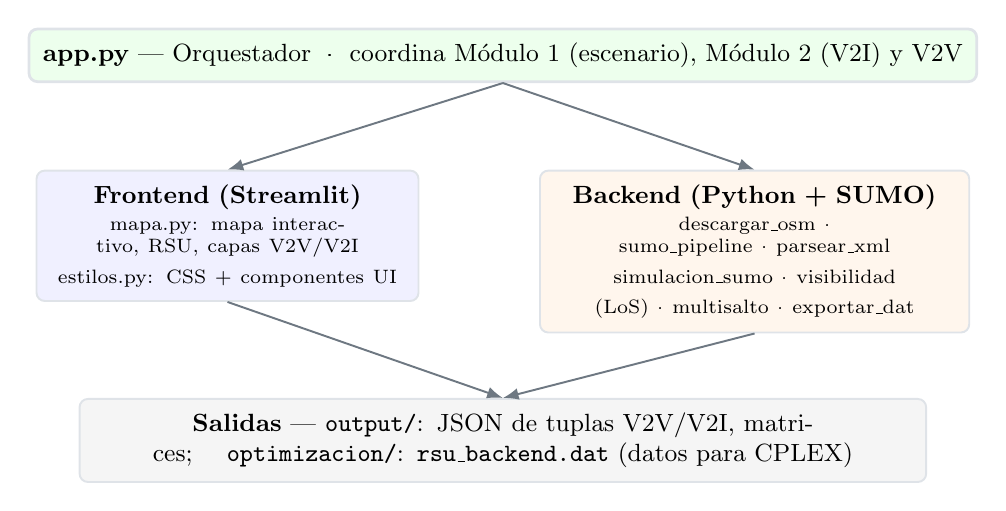
\begin{tikzpicture}[
  font=\small,
  node distance=6mm,
  box/.style={draw=codeframe,line width=0.7pt,rounded corners=3pt,
              align=center,inner sep=5pt,fill=white},
  front/.style={box,fill=blue!6},
  back/.style={box,fill=orange!7},
  orch/.style={box,fill=green!7,line width=1pt},
  outbox/.style={box,fill=gray!8},
  arr/.style={-{Latex[length=2mm]},codecom,line width=0.7pt}
]
\node[orch,minimum width=11.6cm] (orq) {\textbf{app.py} — Orquestador \;·\; coordina Módulo 1 (escenario), Módulo 2 (V2I) y V2V};

\node[front,below right=11mm and 1mm of orq.south west,anchor=north west,text width=4.5cm] (fe)
  {\textbf{Frontend (Streamlit)}\\[2pt]
   \scriptsize mapa.py: mapa interactivo, RSU, capas V2V/V2I\\
   estilos.py: CSS + componentes UI};

\node[back,below left=11mm and 1mm of orq.south east,anchor=north east,text width=5.1cm] (be)
  {\textbf{Backend (Python + SUMO)}\\[2pt]
   \scriptsize descargar\_osm · sumo\_pipeline · parsear\_xml\\
   simulacion\_sumo · visibilidad (LoS) · multisalto · exportar\_dat};

\node[outbox,below=40mm of orq,text width=10.4cm] (ot)
  {\textbf{Salidas} — \texttt{output/}: JSON de tuplas V2V/V2I, matrices; \quad
   \texttt{optimizacion/}: \texttt{rsu\_backend.dat} (datos para CPLEX)};

\draw[arr] (orq.south) -- (fe.north);
\draw[arr] (orq.south) -- (be.north);
\draw[arr] (fe.south) -- (ot.north);
\draw[arr] (be.south) -- (ot.north);
\end{tikzpicture}
\caption{Arquitectura general de la plataforma. El orquestador coordina el
\emph{frontend} de presentación y el \emph{backend} de procesamiento; ambos
convergen en las salidas, entre ellas el conjunto de datos para
optimización.\label{fig:arq}}
\end{figure}

\subsection{Frontend (Streamlit)}
El \emph{frontend} usa Streamlit con mapas Folium embebidos mediante
\texttt{streamlit-folium}. El usuario dibuja un \emph{bounding box} sobre un mapa
real (herramienta \texttt{Draw}); la aplicación captura las cuatro coordenadas y
las envía al \emph{backend}. Los resultados ---RSU candidatas, edificios, matrices
y grafos de conectividad--- se visualizan en capas Folium conmutables y en tablas
interactivas (\texttt{pandas}).

\subsection{Backend (Python + SUMO)}
El \emph{backend} es donde ocurre el trabajo pesado. Llama a las herramientas de
línea de comandos de SUMO como subprocesos y se encarga de todo el cálculo
geométrico y algebraico que viene después (se detalla en la
Sección~\ref{sec:matrices}). El recorrido es el esperable: primero baja los datos del
área con la API de OpenStreetMap; después \texttt{netconvert} y \texttt{polyconvert}
los convierten en la red vial y en los edificios; a continuación
\texttt{randomTrips.py} genera las rutas de los vehículos; y, por último, la
simulación deja un archivo de \emph{Floating Car Data} (FCD) con la posición de cada
vehículo en cada instante.

\subsection{Motor de procesamiento}
A partir de ese FCD, el motor de procesamiento (módulos \texttt{visibilidad.py} y
\texttt{multisalto.py}) es el que arma las matrices de conectividad. Se apoya en
NumPy para toda el álgebra ---productos de matrices, binarización, unión con la
identidad--- y en un detector de línea de vista basado en el test de orientación
CCW, al que se le añaden un par de atajos (pre-filtrado por distancia y por
\emph{bounding box}) para no tener que comparar todo contra todo.

\subsection{Exportación de datos}
La última etapa (\texttt{exportar\_dat.py}) traduce esas matrices al idioma que
entiende el modelo de optimización: los conjuntos de escenarios, vehículos y RSU, los
parámetros de costo, capacidad y penalización, y las tuplas de conectividad
$\langle s,h,v,r\rangle$. La Sección~\ref{sec:export} entra en el detalle.

\begin{figure}[H]
\centering
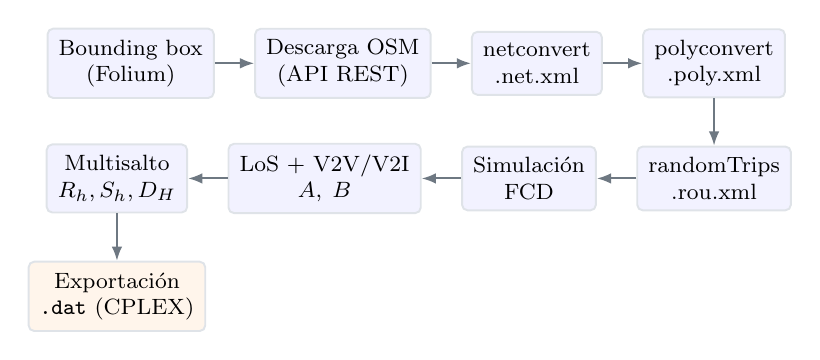
\begin{tikzpicture}[
  font=\footnotesize,
  stg/.style={draw=codeframe,line width=0.7pt,rounded corners=2pt,
              align=center,inner sep=4pt,minimum height=8mm,fill=blue!5},
  arr/.style={-{Latex[length=1.8mm]},codecom,line width=0.7pt}
]
\node[stg] (a) {Bounding box\\(Folium)};
\node[stg,right=5mm of a] (b) {Descarga OSM\\(API REST)};
\node[stg,right=5mm of b] (c) {netconvert\\.net.xml};
\node[stg,right=5mm of c] (d) {polyconvert\\.poly.xml};
\node[stg,below=6mm of d] (e) {randomTrips\\.rou.xml};
\node[stg,left=5mm of e] (f) {Simulación\\FCD};
\node[stg,left=5mm of f] (g) {LoS + V2V/V2I\\$A,\;B$};
\node[stg,left=5mm of g] (h) {Multisalto\\$R_h,S_h,D_H$};
\node[stg,below=6mm of h,fill=orange!8] (i) {Exportación\\\texttt{.dat} (CPLEX)};
\draw[arr] (a)--(b); \draw[arr] (b)--(c); \draw[arr] (c)--(d);
\draw[arr] (d)--(e); \draw[arr] (e)--(f); \draw[arr] (f)--(g);
\draw[arr] (g)--(h); \draw[arr] (h)--(i);
\end{tikzpicture}
\caption{Flujo de procesamiento reproducible: de la selección del área real hasta
el conjunto de datos para optimización.\label{fig:pipeline}}
\end{figure}

%----------------------------------------------------------------------------------
\section{Generación de Matrices de Conectividad}\label{sec:matrices}

La generación de las matrices de conectividad se basa en analizar la red en cada
instante de muestreo $t$ (\emph{snapshot}). En cada uno de estos instantes se registra
el estado de la conectividad entre los nodos mediante matrices de adyacencia binarias.
Sean $\mathcal{V}=\{v_1,\dots,v_n\}$ el conjunto de vehículos activos en ese instante
y $\mathcal{R}=\{r_1,\dots,r_m\}$ el conjunto de RSU candidatas.

\subsection{Matriz V2V ($A$)}
La matriz $A\in\{0,1\}^{n\times n}$ representa la conectividad entre vehículos, donde
$A_{ij}=1$ cuando $v_i$ y $v_j$ mantienen comunicación directa; es decir, ambos se
encuentran dentro del alcance del OBU y ningún edificio obstruye la línea de vista
entre ellos, representada por el segmento $\overline{v_i v_j}$. Dado que este enlace
es bidireccional, la matriz se fuerza a ser simétrica mediante
$A \leftarrow \bin{A \vee A^{\top}}$, donde $\beta(\cdot)$ denota la operación de
binarización aplicada elemento a elemento.

\subsection{Matriz V2I ($B$)}
La matriz $B\in\{0,1\}^{n\times m}$ describe la conectividad entre los vehículos y
las RSU. En particular, $B_{ik}=1$ cuando el vehículo $v_i$ puede comunicarse
directamente con la RSU $r_k$, es decir, se encuentra dentro del alcance del OBU y
existe línea de vista entre ambos. Estas relaciones corresponden a las tuplas de
visibilidad $\langle t, v, r\rangle$ de un solo salto. Para determinar la existencia
de línea de vista se emplea el test de orientación CCW:
\begin{equation}
\mathrm{CCW}(A,B,C) = (B_x-A_x)(C_y-A_y) - (B_y-A_y)(C_x-A_x),
\end{equation}
según el cual dos segmentos se intersectan cuando sus extremos quedan ubicados en
lados opuestos. De este modo, un par $(v,r)$ se descarta tan pronto como alguna
arista de un edificio interseca el segmento $\overline{v r}$.

\subsection{Conectividad multisalto}
Un vehículo que no dispone de conectividad directa con una RSU todavía puede acceder
a ella a través de otros vehículos que actúan como nodos de reenvío. Para modelar
este comportamiento se define la matriz de adyacencia aumentada con la identidad,
$\Atil = A \vee I$, y, a partir de ella, dos familias de matrices: las
\emph{acumuladas} $R_h$ y las de \emph{primera aparición} $S_h$:
\begin{align}
R_1 &= B, & R_h &= \bin{\Atil \, R_{h-1}}, \quad h=2,\dots,H, \label{eq:Rh}\\
S_1 &= R_1, & S_h &= R_h - R_{h-1}, \label{eq:Sh}\\
D_H &= J - R_H, & d_i &= \textstyle\prod_{k}\left(1-(R_H)_{ik}\right), \label{eq:DH}
\end{align}
donde $J$ es la matriz de unos y $d_i=1$ indica que el vehículo $v_i$ no puede
alcanzar ninguna RSU incluso después de considerar hasta $H$ saltos. La inclusión de
la identidad en $\Atil$ desempeña un papel fundamental, ya que garantiza la propiedad
de monotonía $R_1 \le R_2 \le \dots \le R_H$. Si la identidad no se incorporara, el
producto $A\,R_{h-1}$ contabilizaría únicamente los caminos de longitud
\emph{exactamente} $h$, descartando las conexiones de menor longitud que ya habían
sido identificadas en iteraciones anteriores.

\begin{Proposition}\label{prop:caminos}
Sea $\Atil = A\vee I$ y $R_h=\bin{\Atil\,R_{h-1}}$ con $R_1=B$. Entonces
$(R_h)_{ik}=1$ si y solo si existe un camino de \emph{a lo sumo} $h$ saltos que
lleva del vehículo $v_i$ a la RSU $r_k$ en el grafo del \emph{snapshot} (un salto
V2V por cada arista de $A$ recorrida, más el salto V2I final de $B$).
\end{Proposition}

\begin{proof}
Por inducción sobre $h$. \emph{Base} ($h=1$): $R_1=B$ y $B_{ik}=1$ codifica
exactamente el enlace directo $v_i\!\to\!r_k$ de un salto. \emph{Paso inductivo}:
supóngase la tesis para $h-1$. Como $\Atil=A\vee I$, la entrada
$(\Atil\,R_{h-1})_{ik}=\sum_{j}\Atil_{ij}(R_{h-1})_{jk}$ es positiva si y solo si
existe $j$ con $\Atil_{ij}=1$ y $(R_{h-1})_{jk}=1$. Hay dos casos: (i) $j=i$
(término identidad), que arrastra cualquier camino de $\le h-1$ saltos de $v_i$ a
$r_k$; o (ii) $j\neq i$ con $A_{ij}=1$, que antepone un salto V2V $v_i\!\to\!v_j$ a
un camino de $\le h-1$ saltos de $v_j$ a $r_k$, formando un camino de $\le h$
saltos. Aplicando $\beta(\cdot)$ se obtiene $(R_h)_{ik}=1$ exactamente cuando
existe tal camino de a lo sumo $h$ saltos. $\qquad$
\end{proof}

De aquí sale, casi de regalo, la lectura de $S_h=R_h-R_{h-1}$: marca los pares
$(v_i,r_k)$ que aparecen \emph{por primera vez} al salto $h$, es decir, aquellos cuyo
número \emph{mínimo} de saltos es justo $h$. Esa es la semántica exacta que después
consume el modelo de optimización (Sección~\ref{sec:export}). El
Listado~\ref{lst:multisalto} muestra que todo esto cabe en unas pocas líneas de
NumPy.

\begin{lstlisting}[language=Python,caption={Núcleo del cálculo multisalto (NumPy):
identidad, potencias binarias y primera aparición.},label={lst:multisalto}]
def binarizar(X):
    return (X > 0).astype(int)          # beta(X)

def agregar_identidad(A):
    return binarizar(A + np.eye(len(A), dtype=int))   # A_tilde = A v I

def calcular_R(A_tilde, B, H):
    R = [B.copy()]                      # R_1 = B
    for h in range(2, H + 1):
        R.append(binarizar(A_tilde @ R[-1]))          # R_h = beta(A_tilde . R_{h-1})
    return R

def calcular_S(lista_R):
    S = [lista_R[0].copy()]             # S_1 = R_1
    for h in range(1, len(lista_R)):
        S.append(binarizar(lista_R[h] - lista_R[h-1]))# S_h = R_h - R_{h-1}
    return S
\end{lstlisting}

\paragraph{Ejemplo resuelto.} Con $n=4$ vehículos, $m=3$ RSU y $H=3$, dadas
\[
A=\left(\begin{smallmatrix}0&1&0&0\\1&0&1&0\\0&1&0&0\\0&0&0&0\end{smallmatrix}\right),\quad
B=\left(\begin{smallmatrix}1&0&0\\0&0&1\\0&1&0\\0&0&0\end{smallmatrix}\right),
\]
la plataforma devuelve $R_3$, $S_2$, $S_3$ y el vector $d$, que se muestran como mapa
de calor en la Figura~\ref{fig:heat}. La lectura es intuitiva: $v_1$, $v_2$ y $v_3$
terminan alcanzando las tres RSU en $\le 3$ saltos ---por ejemplo,
$v_1\!\to\!v_2\!\to\!v_3\!\to\!r_2$ es un camino de tres saltos que asoma en $S_3$---,
mientras que $v_4$, sin un solo enlace, se queda completamente aislado ($d_4=1$).

\begin{figure}[H]
\centering
\newcommand{\hc}[1]{\ifnum#1=1\cellcolor{blue!55}\textcolor{white}{1}\else\cellcolor{gray!8}0\fi}
\small
\begin{tabular}{c@{\hskip 8mm}c@{\hskip 8mm}c}
% ---- R3 ----
\begin{tabular}{c|ccc}
$R_3$ & $r_1$ & $r_2$ & $r_3$\\\hline
$v_1$ & \hc1 & \hc1 & \hc1\\
$v_2$ & \hc1 & \hc1 & \hc1\\
$v_3$ & \hc1 & \hc1 & \hc1\\
$v_4$ & \hc0 & \hc0 & \hc0\\
\end{tabular}
&
% ---- S2 ----
\begin{tabular}{c|ccc}
$S_2$ & $r_1$ & $r_2$ & $r_3$\\\hline
$v_1$ & \hc0 & \hc0 & \hc1\\
$v_2$ & \hc1 & \hc1 & \hc0\\
$v_3$ & \hc0 & \hc0 & \hc1\\
$v_4$ & \hc0 & \hc0 & \hc0\\
\end{tabular}
&
% ---- S3 ----
\begin{tabular}{c|ccc}
$S_3$ & $r_1$ & $r_2$ & $r_3$\\\hline
$v_1$ & \hc0 & \hc1 & \hc0\\
$v_2$ & \hc0 & \hc0 & \hc0\\
$v_3$ & \hc1 & \hc0 & \hc0\\
$v_4$ & \hc0 & \hc0 & \hc0\\
\end{tabular}
\end{tabular}
\caption{Mapas de calor de la conectividad multisalto correspondientes al ejemplo
resuelto ($H=3$). La parte izquierda muestra el alcance acumulado $R_3$, mientras
que las secciones central y derecha representan las conexiones que aparecen por
primera vez a 2 ($S_2$) y 3 ($S_3$) saltos, respectivamente. La ausencia de valores
en la fila asociada a $v_4$ dentro de $R_3$ indica que el vehículo no alcanza ninguna
RSU en el límite considerado, por lo que $d_4=1$ y se clasifica como aislado.
\label{fig:heat}}
\end{figure}

%----------------------------------------------------------------------------------
\section{Selección de Posiciones Candidatas para RSU}\label{sec:rsu}

\subsection{Justificación de la reducción}
Al importar un archivo OSM, SUMO genera un conjunto amplio de
\emph{junctions}; sin embargo, una parte de estos nodos no corresponde a ubicaciones
viables para el despliegue de RSU. Dentro de este conjunto pueden encontrarse puntos
intermedios de una vía, bifurcaciones asociadas a caminos secundarios o conexiones
menores que no representan intersecciones relevantes para la infraestructura
vehicular. Por esta razón, el proceso de selección considera únicamente aquellas
intersecciones con mayor relevancia desde el punto de vista del tránsito, donde
convergen varias vías y pueden producirse cambios en la trayectoria o velocidad de
los vehículos.

Este filtrado permite reducir de manera considerable el espacio de búsqueda para la
ubicación de RSU. En el escenario evaluado, las 620 \emph{junctions} generadas
inicialmente por SUMO fueron reducidas a 160 posiciones candidatas, equivalente a
una disminución del 74\,\%, manteniendo aquellas intersecciones con mayor potencial
para la instalación de infraestructura.

\subsection{Algoritmo principal}
El proceso de selección se desarrolla en dos fases complementarias. En la primera se
realiza un filtrado topológico basado en el \emph{grado} de cada nodo, considerando
la cantidad de calles conectadas (aristas no internas) y eliminando aquellas
posiciones con un nivel de conectividad reducido. Posteriormente, se aplica un
\emph{clustering} espacial de tipo \emph{greedy} sobre las posiciones restantes,
con el propósito de agrupar candidatos ubicados a distancias reducidas y conservar
en cada grupo aquel nodo que presenta el mayor grado topológico.

El Listado~\ref{lst:rsu} muestra el pseudocódigo del procedimiento implementado en
\texttt{filtrar\_junctions\_rsu()}. La estructura planteada permite extender el
método con otros criterios de selección de RSU, como enfoques basados en cobertura o
en centralidad de intermediación, utilizando el mismo conjunto de datos de entrada
y facilitando la comparación entre diferentes estrategias de despliegue.

\begin{lstlisting}[caption={Pseudocódigo del algoritmo de selección de RSU
candidatas (filtro por grado + \emph{clustering} greedy).},label={lst:rsu}]
Entrada:  junctions J, aristas E, grado_min g, radio_cluster rho
Salida:   candidatas C

// Etapa 1 - Filtro topologico por grado
para cada arista e en E:
    si e.function == "internal":  continuar        // ignorar aristas internas
    grado[e.from] += 1;  grado[e.to] += 1
F <- { j en J : grado[j] >= g }                     // sobreviven grado >= g

// Etapa 2 - Clustering espacial greedy
ordenar F por grado DESCENDENTE
C <- {}
para cada j en F:                                   // de mayor a menor grado
    d_min <- min_{c en C} distancia_euclidiana(j, c)
    si C == {}  o  d_min > rho:
        C <- C union {j}                            // nueva RSU candidata
    // si no: se descarta (ya hay un centro cercano de mayor grado)
retornar C
\end{lstlisting}

Una ventaja práctica de este enfoque es que las coordenadas generadas por SUMO se
expresan directamente en metros (UTM con \emph{offset}), por lo que la distancia
euclidiana $\sqrt{(x_1-x_2)^2+(y_1-y_2)^2}$ corresponde a la distancia real, sin
necesidad de realizar conversiones adicionales. Tanto el grado mínimo (valor
predeterminado de 4) como el radio de \emph{clustering} (20\,m por defecto) pueden
configurarse desde la interfaz.

%----------------------------------------------------------------------------------
\section{Exportación de Datos para Optimización}\label{sec:export}

Una vez construidas las matrices de conectividad, el siguiente paso consiste en
transformarlas en un formato que pueda ser utilizado por un \emph{solver} de
optimización. Para ello, el módulo \texttt{exportar\_dat.py} toma las matrices $S_h$
y las convierte en la entrada del modelo estocástico de despliegue de RSU. La
conversión es directa: cada instante de muestreo $t$ se representa como un
\emph{escenario} $s$, mientras que cada valor igual a $1$ en $S_h[v][r]$ se traduce
en una tupla $\langle s,h,v,r\rangle$, que conforma el conjunto \texttt{CVR}.

Con el fin de garantizar que el modelo siempre disponga de una solución factible, los
vehículos que no logran establecer conexión con ninguna RSU real se asocian a una RSU
artificial $r_\infty$ (identificador $0$) en el salto
$h_{\max}=H+1$, asignándoles una penalización elevada. El
Listado~\ref{lst:dat} presenta un extracto del archivo \texttt{.dat} generado,
compatible con OPL/CPLEX. Además, la misma información se construye en memoria para
ser utilizada por \emph{solvers} de Python, como \texttt{docplex}.

\begin{lstlisting}[language=opldat,caption={Extracto del conjunto de datos exportado
(\texttt{rsu\_backend.dat}) en sintaxis OPL, con cabecera de trazabilidad
escenario$\to t$ y RSU$\to$id de \emph{backend}.},label={lst:dat}]
// escenario s=1  ->  t=120.0     |  RSU OPL 1..m sobre sorted(rsus)
hmax = 4;            // H+1: el ultimo salto es el RSU artificial
rInf = 0;           // RSU de "desconexion"
MaxR = 5;           // maximo de RSU reales a desplegar
R = { 0 1 2 3 ... }; S = { 1 2 3 }; V = { 0 1 2 ... };
Vs = [ {0 1 2 ...} {1 2 ...} {...} ];      // vehiculos por escenario
P = [ 1 2 4 1000 ];                        // penalizacion por saltos
CVR = {
  <1, 1, 0, 12>   // esc.1: v0 alcanza RSU 12 con 1 salto
  <1, 2, 3, 7>    // esc.1: v3 alcanza RSU 7  con 2 saltos (multisalto)
  <1, 4, 0, 0>    // esc.1: v0 cae en r_inf (desconectado)
  ...
};
\end{lstlisting}

Este archivo desacopla la simulación del \emph{solver}: los mismos conjuntos y
parámetros pueden alimentar distintas formulaciones (\emph{p-median}, cobertura,
etc.) sin volver a simular.

%----------------------------------------------------------------------------------
\section{Caso de Estudio}\label{sec:caso}

\subsection{Escenario SUMO}
Se seleccionó una zona del Centro Histórico de Quito (Ecuador). La
Tabla~\ref{tab:caso} resume las magnitudes del escenario tras ejecutar el
\emph{pipeline} completo.

\begin{table}[H]
\caption{Magnitudes del caso de estudio (Centro Histórico de Quito).\label{tab:caso}}
\begin{tabularx}{\textwidth}{Xr}
\toprule
\textbf{Magnitud} & \textbf{Valor}\\
\midrule
\emph{Junctions} generadas por SUMO & 620\\
RSU candidatas tras filtrado (grado + \emph{clustering}) & 160 (\,$-74\%$\,)\\
Vehículos simulados & 132\\
Instantes de muestreo (escenarios $s$) & 31\\
RSU con al menos un vehículo conectado & 256--333\\
Tuplas de conectividad $\langle s,h,v,r\rangle$ (\texttt{CVR}) & 1\,710\\
Tiempo de cálculo LoS + matrices & $<5$ s\\
\bottomrule
\end{tabularx}
\end{table}

\subsection{Resultados de conectividad multisalto}
La evolución de la cobertura por número de saltos muestra el aporte del reenvío
multisalto: pares $(v,r)$ que no existen a un salto ($B$) aparecen a 2 y 3 saltos
gracias a los vehículos repetidores, y el vector $d$ identifica los vehículos que
permanecen aislados aun con $H$ saltos. Estos resultados se visualizan en la
plataforma como tablas y mapas de calor (cf.\ Figura~\ref{fig:heat} para el ejemplo
canónico).

\subsection{Ejemplo de exportación}
La plataforma exportó el conjunto de datos de la Tabla~\ref{tab:caso} al archivo
\texttt{rsu\_backend.dat} (extracto en el Listado~\ref{lst:dat}), directamente
consumible por un \emph{solver} de optimización. Con ello se cierra el ciclo
Escenario SUMO~$\rightarrow$~matrices~$\rightarrow$~datos para optimización sin
intervención manual.

%----------------------------------------------------------------------------------
\section{Discusión}

\textbf{Ventajas.} La plataforma reúne en un mismo flujo de trabajo todas las etapas
necesarias para obtener los datos de conectividad. En lugar de ejecutar varios
\emph{scripts} independientes para simular el tráfico, calcular la línea de vista,
generar las matrices y preparar la información para el modelo de optimización, todo
el proceso se realiza de forma integrada. Esto facilita la reproducción de los
experimentos, ya que una misma configuración de entrada definida mediante el
\emph{bounding box} genera el mismo conjunto de datos en ejecuciones sucesivas.

Otro aspecto relevante es la separación entre la simulación y el modelo de
optimización. Las matrices de conectividad se generan en un formato independiente,
por lo que pueden emplearse posteriormente en distintos modelos, ya sean exactos o
heurísticos, sin necesidad de repetir la simulación. Además, al conservar la
correspondencia entre los escenarios simulados y los instantes de tiempo, así como
entre los identificadores de las RSU y su ubicación real, es posible representar los
resultados del \emph{solver} directamente sobre el mapa e interpretarlos con mayor
facilidad.

\textbf{Limitaciones.} La implementación actual también presenta algunas
restricciones. La transformación de las coordenadas internas de SUMO a latitud y
longitud se basa en una interpolación lineal, una aproximación adecuada para áreas
de tamaño reducido ($<10$\,km$^2$), aunque menos precisa cuando el escenario cubre
regiones más extensas. En esos casos sería preferible utilizar una proyección
cartográfica específica.

Asimismo, el análisis de línea de vista considera únicamente la geometría
bidimensional de los edificios, representándolos como polígonos sin altura. Como
consecuencia, no se modelan fenómenos propios de la propagación inalámbrica, tales
como la atenuación de la señal o el multitrayecto, por lo que la conectividad
estimada debe entenderse como una aproximación geométrica. Finalmente, cada
\emph{snapshot} se procesa de forma independiente, sin contemplar la evolución
temporal de la conectividad ni la latencia asociada al reenvío de mensajes.

\textbf{Trabajo futuro.} Existen varias posibilidades para ampliar el alcance de la
plataforma. Entre ellas se encuentran la incorporación de \texttt{pyproj} para
realizar conversiones cartográficas más precisas, la sustitución del modelo binario
de línea de vista por modelos de propagación que consideren pérdidas de trayectoria
(\emph{path loss}) y la evaluación de nuevos criterios para seleccionar posiciones
candidatas de RSU. También resulta de interés integrar la salida del
\emph{solver} en la interfaz de la aplicación, de modo que el despliegue obtenido
pueda visualizarse directamente sobre el mapa.

%----------------------------------------------------------------------------------
\section{Conclusiones}

Este trabajo demuestra que la generación de las matrices de conectividad, un paso que
con frecuencia permanece implícito en los estudios de despliegue de RSU, puede
automatizarse de forma completamente reproducible. A partir de un área real
seleccionada sobre el mapa, la plataforma simula el tráfico mediante SUMO, determina
la conectividad con línea de vista entre pares vehículo--vehículo y
vehículo--RSU, y construye tanto las matrices de conectividad directa como las de
conectividad multisalto, respaldadas por la justificación formal presentada en la
Proposición~\ref{prop:caminos}. Como resultado, se obtiene un conjunto de datos listo
para ser utilizado por modelos de optimización.

El enfoque propuesto concibe este proceso como una etapa de preprocesamiento
independiente del modelo de optimización, de modo que un mismo conjunto de datos
pueda emplearse en diferentes formulaciones sin necesidad de repetir la simulación.
Como trabajo futuro, se plantea integrar estos datos con modelos de optimización,
tanto exactos como heurísticos, con el propósito de abordar no solo la generación de
la información de entrada, sino también la determinación del despliegue óptimo de la
infraestructura vehicular.

%----------------------------------------------------------------------------------
\vspace{6pt}

\authorcontributions{Conceptualización, metodología, software, validación,
redacción---preparación del borrador original y redacción---revisión y edición,
E.X.E.S. El autor ha leído y aceptado la versión publicada del manuscrito.}

\funding{Esta investigación no recibió financiamiento externo.}

\dataavailability{Los datos y el código que respaldan los resultados están
disponibles en el repositorio del proyecto.}

\acknowledgments{El autor agradece el apoyo institucional. Durante la preparación de
este manuscrito se utilizó una herramienta de asistencia basada en IA para la
maquetación de LaTeX y la redacción de borradores; el autor revisó y editó el
contenido y asume la responsabilidad plena de la publicación.}

\conflictsofinterest{El autor declara no tener conflictos de interés.}

\abbreviations{Abreviaturas}{%
En este manuscrito se usan las siguientes abreviaturas:\\

\noindent
\begin{tabular}{@{}ll}
VANET & Vehicular Ad hoc Network\\
V2V   & Vehicle-to-Vehicle\\
V2I   & Vehicle-to-Infrastructure\\
RSU   & Road Side Unit\\
OBU   & On Board Unit\\
LoS   & Line of Sight\\
FCD   & Floating Car Data\\
SUMO  & Simulation of Urban MObility\\
OSM   & OpenStreetMap
\end{tabular}
}

%----------------------------------------------------------------------------------
\reftitle{Referencias}

\begin{thebibliography}{999}
\bibitem{ref-urquiza}
Urquiza-Aguiar, L.; Tripp-Barba, C.; Aguilar-Igartua, M. A Stochastic Optimization
Model for the Placement of Road Side Units. In {\em Proceedings of the ADHOC-NOW};
Springer: Cham, Switzerland, 2016.

\bibitem{ref-sumo}
Lopez, P.A.; Behrisch, M.; Bieker-Walz, L.; et~al. Microscopic Traffic Simulation
using SUMO. In {\em Proceedings of the 21st IEEE ITSC}; IEEE: Maui, HI, USA, 2018;
pp. 2575--2582.

\bibitem{ref-osm}
OpenStreetMap contributors. OpenStreetMap. Available online:
\url{https://www.openstreetmap.org} (accessed on 20 July 2026).

\bibitem{ref-streamlit}
Streamlit Inc. Streamlit: A faster way to build and share data apps. Available
online: \url{https://streamlit.io} (accessed on 20 July 2026).

\bibitem{ref-folium}
python-visualization. Folium: Python Data, Leaflet.js Maps. Available online:
\url{https://python-visualization.github.io/folium/} (accessed on 20 July 2026).
\end{thebibliography}

\PublishersNote{}
\end{document}
